% bare_jrnl_compsoc, texV1.4b, 2015/08/26, Michael Shell
\documentclass[10pt,journal,compsoc]{IEEEtran}

% *** MISC UTILITY PACKAGES ***

\newcommand{\note}[1]{\textcolor{magenta}{#1}} 
\usepackage[nocompress]{cite}
\usepackage[]{footmisc}
\usepackage{hyperref} % autoref
% *** GRAPHICS RELATED PACKAGES ***
\ifCLASSINFOpdf
   \usepackage[pdftex]{graphicx}
  % declare the path(s) where your graphic files are
   \graphicspath{{./figures/}}
  % and their extensions so you won't have to specify these with
  % every instance of \includegraphics
  % \DeclareGraphicsExtensions{.pdf,.jpeg,.png}
\else
  % or other class option (dvipsone, dvipdf, if not using dvips). graphicx
  % will default to the driver specified in the system graphics.cfg if no
  % driver is specified.
   \usepackage[dvips]{graphicx}
  % declare the path(s) where your graphic files are
   \graphicspath{{./figures/}}
  % and their extensions so you won't have to specify these with
  % every instance of \includegraphics
   \DeclareGraphicsExtensions{.eps}
\fi

% latex, and pdflatex in dvi mode, support graphics in encapsulated
% postscript (.eps) format. pdflatex in pdf mode supports graphics
% in .pdf, .jpeg, .png and .mps (metapost) formats. Users should ensure
% that all non-photo figures use a vector format (.eps, .pdf, .mps) and
% not a bitmapped formats (.jpeg, .png). The IEEE frowns on bitmapped formats
% which can result in "jaggedy"/blurry rendering of lines and letters as
% well as large increases in file sizes.

% *** MATH PACKAGES ***
%% with other math-related packages, you may want to disable it.
\usepackage{amsmath, amsthm, amsfonts,amssymb,eulervm,xspace, mathtools}
\usepackage{stmaryrd}%mapsfrom 
\renewcommand{\restriction}{\mathord{\upharpoonright}} %restriction w/p space
\usepackage{mathrsfs} % math script fonts
\usepackage{relsize} %bigger
\usepackage{bm}
\theoremstyle{definition}
\newtheorem{definition}{Definition}[section]
\theoremstyle{remark}
\newtheorem{example}{Example}[section]
% *** SPECIALIZED LIST PACKAGES ***
\usepackage{xcolor}
\usepackage{algorithmic}
\usepackage[utf8]{inputenc}
\usepackage{subfig} %ieee does not like subfigure
\usepackage{multicol}
\usepackage{tikz}
\usetikzlibrary{cd} % commutative diagrams
\newtheorem{axiom}{Axiom}
\newtheorem{prop}{Proposition} %math?
\usepackage[switch]{lineno}
\renewcommand{\linenumberfont}{\normalfont\bfseries\small\color{lightgray}}
\usepackage{minted}
\setminted[python]{fontsize=\scriptsize, 
                   linenos,
                   numbersep=8pt,
                   autogobble, 
                   frame=lines,
                   framesep=3mm} 
% *** ALIGNMENT PACKAGES ***
\usepackage{array}
\usepackage{tabulary}
% IEEEtran contains the IEEEeqnarray family of commands

% *** SUBFIGURE PACKAGES ***
\ifCLASSOPTIONcompsoc
  \usepackage[caption=false,font=footnotesize,labelfont=sf,textfont=sf]{subfig}
\else
  \usepackage[caption=false,font=footnotesize]{subfig}
\fi

% *** FLOAT PACKAGES ***
\usepackage{dblfloatfix}

% *** PDF, URL AND HYPERLINK PACKAGES ***
\usepackage{url}

% *** Do not adjust lengths that control margins, column widths, etc. ***
% *** Do not use packages that alter fonts (such as pslatex).         ***
% There should be no need to do such things with IEEEtran.cls V1.6 and later.
% (Unless specifically asked to do so by the journal or conference you plan
% to submit to, of course. )

\usepackage{notation} %notation conventions
% correct bad hyphenation here
\hyphenation{op-tical net-works semi-conduc-tor}



\begin{document}
\linenumbers

\title{Topological Equivariant Artist Model for Visualization Library Architecture}
% author names and IEEE memberships
\author{Hannah~Aizenman, Thomas~Caswell, and~Michael~Grossberg,~\IEEEmembership{Member,~IEEE,}% <-this % stops a space
\IEEEcompsocitemizethanks{\IEEEcompsocthanksitem H. Aizenman and M. Grossberg are with the department of Computer Science, City College of New York. 
\protect\\
% note need leading \protect in front of \\ to get a newline within \thanks as
% \\ is fragile and will error, could use \hfil\break instead.
E-mail: haizenman@ccny.cuny.edu, mgrossberg@ccny.cuny.edu 
\IEEEcompsocthanksitem Thomas Caswell is with National Synchrotron Light Source II, Brookhaven National Lab 
\protect \\
E-mail: tcaswell@bnl.gov}% <-this % stops an unwanted space
\thanks{Manuscript received X XX, XXXX; revised X XX, XXXX.}
}


% for Computer Society papers, we must declare the abstract and index terms
% PRIOR to the title within the \IEEEtitleabstractindextext IEEEtran
% command as these need to go into the title area created by \maketitle.
% As a general rule, do not put math, special symbols or citations
% in the abstract or keywords.
\IEEEtitleabstractindextext{%
\begin{abstract}
The abstract goes here.
\end{abstract}

% Note that keywords are not normally used for peerreview papers.
\begin{IEEEkeywords}
%Computer Society, IEEE, IEEEtran, journal, \LaTeX, paper, template.
\end{IEEEkeywords}}


% make the title area
\maketitle


\IEEEpeerreviewmaketitle



\IEEEraisesectionheading{\section{Introduction}\label{sec:intro}}


\IEEEPARstart{T}

\section{Related Work}

\section{Data And Visualizations}
\label{sec:atct}
\note{why why why?}
We use concepts from algberaic topolology and category theory to formally express the structure visualization components are expected to preserve.  Fiber bundles and sheaves, which come from algebraic topolology, provide a uniform generalizable way to describe data and visualizations. Category theory is a method to describe how objects are specified, constrained, and composed \cite{wielsManagementEvolvingSpecifications1998}\; therefore in this work we propose categorical constructions of visualization components as specifications for implementable components.

\subsection{Fiber Bundles}
\label{sec:atct:fiber-bundles}
Fiber bundles, are a "unified, dimension-independent framework", as described by Butler\cite{butlerVectorBundleClassesForm1992,butlerVisualizationModelBased1989}, that allow us to seperatly describe the topological properties and fields of a data source and also the mapping between topolology and data values. A fiber bundle $(\dtotalc, \dbasec, \pi, \dfiberc)$ is a structure with topological spaces $\dtotalc, \dfiberc, \dbasec$ and continuous surjective map $\pi: \dtotalc \rightarrow \dbasec$\cite{FiberBundle2020}. 

\begin{equation}[h]
  \label{eq:atct:fb_intro}
  \begin{tikzcd}[ampersand replacement=\&, row sep=huge]
   \dfiberc
    \arrow[r, hook, color=total] \& 
    \dtotalc
    \arrow[d, "\pi"',color=total] \\
     \& 
  \dbasec
     \arrow[u, "\dsectionc"', bend right, pos=.5, color=section]
  \end{tikzcd}
\end{equation} 

The \textcolor{base}{base space} is a topological space \dbasec\ with points $\dbasepointc \in \dbasec$ and topology $\mathcal{T}_{\dbasec}$; $\mathcal{T}_k$ is a set of opensets $ \dbasepointc \in \opensetc \subseteqq \dbasec$ \cite{munkresElementsAlgebraicTopology1984} that cover the base space \dbasec.  The \textcolor{fiber}{fiber space} is a topological space \dfiberc\ that is the preimage of the projection function $\pi$ at a point in the base space $\dfiber_{\dbasepointc} = \pi^{-1}(\dbasepointc)$ and fibers of a bundle are isomorphic $\dfiberc \simeq \dfiberc_{\dbasepointc}\;\forall \dbasepointc \in \dbase$. The \textcolor{section}{sections} of a bundle $\dsection$ are maps from the base space to points in the bundles over that base space and $\textcolor{set}{\Gamma}$ denotes the set of all sections in a bundle over an openset. 
\begin{equation}
  \label{eq:atct:fb_sections}
  \cgamma{\opensetc}{\dtotalc\restriction_{\opensetc}} \coloneqq \big\{\dsectionc: \opensetc\rightarrow \dtotalc\restriction_{\opensetc} \; \bigm{\vert} \pi(\dsectionc(\dbasepointc)) = \dbasepointc\;for\, all\; \dbasepointc \in \opensetc \big\} 
\end{equation}
 
A fiber bundle is locally trivial, which means that for every point \dbasepointc\ there exists an open neighborhood $\dbasepointc \in \opensetc \subseteq \dbasec$ such that there is a homeomorphism $\pi^{-1}(\opensetc)\xrightarrow{\equivc} \opensetc \times \dfiberc$. A bundle may be globally trivial, meaning that $\dtotalc = \dbasec \times \dfiberc$, and generally can be thought of as a twisted product of total and base spaces \cite{munkresElementsAlgebraicTopology1984}. 

\begin{figure}[h]
  \label{fig:atct:fb}
  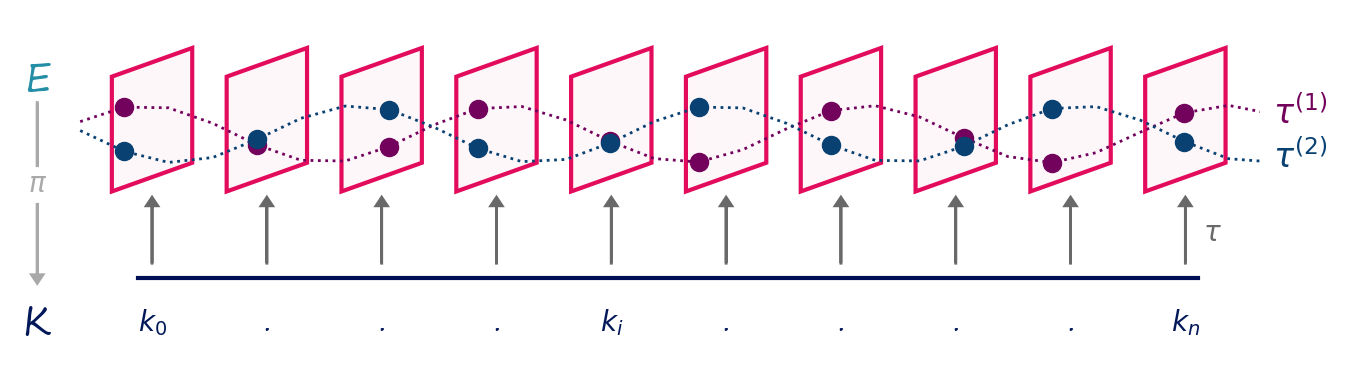
\includegraphics[width=\columnwidth]{fiberbundle.png}
  \caption{change to concrete example}
\end{figure}

Fiber bundles can be used to model data for visualization, as proposed by Butler\cite{butlerVectorBundleClassesForm1992, butlerVisualizationModelBased1989}. We describe the topological properties of the data \cite{wilkinsonGrammarGraphics2005} as the base space \dbasec. The topological properties, as described by Wilkenson, are how the data is organized - for example \dbase\ could be discrete points, a line, a 2D surface, a 3D volume, or a graph. The names and data types of the data fields can be expressed as the fiber space \dfiberc, as described by Spivak \cite{spivakDatabasesAreCategories2010,spivakSIMPLICIALDATABASES}. For example, a temperature field could be expressed as a fiber $\dfiber_{temperature}=\mathbb{R}$, and a color field could be $\dfiber_{color}=\mathbb{R}^{3}$. Even though fibers on non-trivial spaces, such as vector fields, are different, we can simplify to one type because fibers are isomorphic.\note{unsure of this claim but I think this is why, and also I need to tell you why you care that they're isomorphic} The total bundle space \dtotalc\ acts as a way of expressing all data with the same topology \dbasec\ and fields \dfiberc, for example a database schema. A specific dataset is represented as a section \dsectionc, and the return values of a section evaluated at a point \dbasepointc\ is the record $\{field_{0}: value_{0}, ..., field_n:value_n\}$ at that point. 

\begin{figure}
  \label{fig:atct:fb_graphic_bundle}
  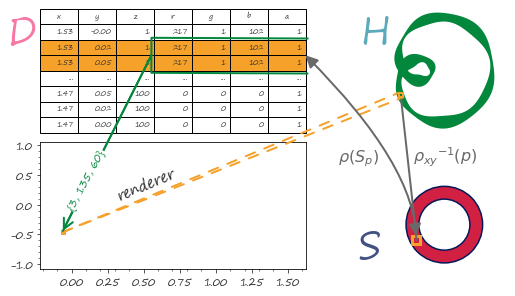
\includegraphics[width=1\columnwidth]{render.png}
  \caption{}
\end{figure}

We also use fiber bundles to represent the output of a visualization algorithm, which we term the graphic but generalizes to output on any display space, such as a screen or 3D print. 
\begin{equation}
  \label{eq:atct:fb_graphic}
  \gfiberc \hookrightarrow \gtotalc \xrightarrow{\pi} \gbasec
\end{equation}
The base space \gbasec\ is a parameterization of the display area, for example the inked bounding box in cairo \cite{CairographicsOrg}. The fiber space \gfiberc\ is an abstraction of the renderer fields, for example $\{x,\,y,\,r,\,g,\,b,\,a\}$. The sections of the graphic 
\begin{equation}
  \label{eq:atct:fb_graphic_section}
  \cgamma{\opensetgc}{\gtotalc\restriction_{\opensetgc}} \coloneqq \big\{\gsectionc: \opensetgc\rightarrow \gtotalc\restriction_{\opensetgc} \; \bigm{\vert} \pi(\gsectionc(\gbasepointc)) = \gbasepointc\;for\, all\; \gbasepointc \in \opensetgc \big\}
\end{equation}
are functions that generate different graphics, for example markers for a scatter plot, bars for a bar chart, cells of a heatmap, or pixels of an image.

\subsection{Input and Output Types}
\label{sec:atct:io}
As described in \autoref{sec:atct:fiber-bundles}, we model data as a map from base space to fiber space.To encapsulate the structure carried in these maps, and provide a way to define these maps in reusable and composable manner, we define categories of base and fiber spaces. 

\begin{definition}
  \label{sec:atct:io:base}
  The base space category $\mathcal{\opensetc}$ has open set objects $\opensetc$ and inclusion morphisms $\iota: \opensetc_1 \rightarrow \opensetc_2$ such that $\opensetc_1 \subseteq \opensetc_2$. 
\end{definition}

By definition, each object in a category has an identity morphism and morphisms are associative and commutative \cite{barrCategoryTheoryComputing}. 

\begin{definition}
  \label{def:atct:io:fiber}
  The fiber category $\mathcal{\dfiberc}$ is a monoidal category, meaning the category has a single object $\dfiberc$ of an arbitrary type. The morphisms on the fiber object are $\dfunctc \in Hom(\dfiberc, \dfiberc)$. 
\end{definition}

The fiber category is equipped with a bifunctor $\otimes: \mathcal{\dfiber} \times {\dfiber}$. The bifunctor provides a method for combining fibers, thereby allowing for fields that contain multityped values. For example, RGB color can either be represented as three fiber fields $\dfiber_{red}, \dfiber_{green}, \dfiber_{blue}$ or a composite fiber field $\dfiber_{red} \otimes \dfiber_{green} \otimes \dfiber_{blue} = \dfiber_{RGB}$.

\subsection{Sheaves}
Sheaves on bundles are an "algebraic data structure", as described by Ghrist \cite{ghristElementaryAppliedTopology2014}, for expressing the bookkeeping involved in keeping track of sections of data over opensets. Sheaves are a way of expressing that subsets, distributed data, and streaming data are local sections that can be glued together. Formally, pre-sheaves are functors, meaning they are functions from objects of one category to objects of another category \cite{WhatFunctorDefinitions}. Here the sheaf 
\begin{equation}
  \sheafc_{\dbasec, \dtotalc}: \opensetc \rightarrow \cgamma{\opensetc}{\dtotalc\restriction_{\opensetc}}
\end{equation}
denotes a sheaf from opensets on the base space $\dbase$ to sets of sections on the bundle $\dtotal$. As a contravariant functor it preserves morphism s

\begin{equation}
  \label{eq:atct:presheaf}
  \begin{tikzcd}
    \cgamma{\opensetc_1}{\dtotalc\restriction_{\opensetc_1}}  &  & \cgamma{\opensetc_2}{\dtotalc\restriction_{\opensetc_2}} 
    \arrow[ll, "\iota^*"', maps to, color=set] \\
    & & \\
    \opensetc_1 
    \arrow[rr, "\iota", maps to, color=base] 
    \arrow[uu, "{\sheafc_{\dbasec, \dtotalc}}", maps to, color=sheaf] &  & \opensetc_2 
    \arrow[uu, "{\sheafc_{\dbasec, \dtotalc}}"', maps to, color=sheaf]              
    \end{tikzcd}
\end{equation}

which associates a set of sections $\cgamma{\openset}{\dtotal\restriction_{\openset}}$ with an openset \openset. The sets of sections are objects of the category \setc\ and the morphisms of the category are restrictions\footnote{restriction functions } $\iota^*$. The sheaf over a an open set $\openset$ surrounding a point $\dbasepoint$ is called a stalk\cite{StalkSheaf2019}
\begin{equation}
  \label{eq:atct:sheaf:stalk}
    \sheaf_{\dbase, \dtotalc}\restriction_{\dbasepoint}\coloneqq \lim\limits_{\openset\ni \dbasepoint} \Gamma(\openset, \dtotal\restriction_{\openset}) 
\end{equation}
where the fiber is contained inside the stalk  $\dfiber_{\dbasepoint} \subset  \sheaf_{\dbase, \dtotal}\restriction_{\dbasepoint}$. The germ is the section evaluated at a point in the stalk  $\dsection(\dbasepoint) \in \sheaf_{\dbase, \dtotal}\restriction_{\dbasepoint}$ and is the data. \note{I never use stalk and germ terminology at any point in this paper}
 
A sheaf is a presheaf that satisfies the locality and gluing axioms \cite{bakerMathsSheaf}. The locality axiom is that given a union of opensets $\mathscr{\opensetc} = \bigcup\limits_{i\in I} \opensetc_i$ and $\dsectionc^{a}, \dsectionc^{b} \in \sheafc(\mathscr{\opensetc})$,  if $\dsectionc^{a}\restriction_{\opensetc_i} = \dsectionc^{b}\restriction_{\opensetc_i}$ for each $\opensetc_i \in \opensetc$ then $\dsectionc^{a} = \dsectionc^{b}$. This means that two sections in a sheaf are equal when they evaluate to the same values over all open sets in a collection. The gluing axiom is that given $\dsectionc^{i} \in \sheafc(\opensetc_i)$ such that ${\dsectionc^{i}}\restriction_{\opensetc_i\cap \opensetc_j} = {\dsectionc^{j}}\restriction_{\opensetc_i \cap \opensetc_j}$ for $\opensetc_i, \opensetc_j \in \mathscr{\opensetc}$, there exists $\dsectionc \in \sheafc(\mathscr{\opensetc})$ such that $\dsectionc\restriction_{\opensetc_i} = {\dsectionc^{i}}$. This means we can construct a section $\dsection$ on the collection of open sets that is the union of sections defined on specific open sets. This expresses an equivalency between a concatenated represetation of data and the distributed representation of the same data. 

In this model, we represent data and graphics as a sheaf; doing so allows us to express that data sources are expected to have the bookkeeping that a sheaf requires, meaning inclusions, restrictions, locality, and gluing must be preserved. 

\subsubsection{Measurement Scales}
\label{sec:atct:sheaves:measurments}
We specify that structure on a sheaf includes the actions $\dfuncc$ on sections of that sheaf, which is a generalization of Steven's \cite{stevensTheoryScalesMeasurement1946} classification of measurement scales by their mathematical group structure. These sheaf actions describe which changes in the data we expect to be equivariant to changes in the visualization. 

\begin{equation}
  \label{eq:atct:sheaves:monoid_morphism}
  \begin{tikzcd}
    \cgamma{\opensetc}{\dtotalc\restriction_{\opensetc}} 
    \arrow[rr, "\dfuncpullc", color=action, maps to] &  & 
    \cgamma{\opensetc^{\prime}}{\dfuncpullc\dtotalc\restriction_{\opensetc^{\prime}}} & 
    \cgamma{\opensetc^{\prime}}{\dfuncpullc\dtotalc\restriction_{\opensetc^{\prime}}} 
    \arrow[dd, "\dfunctc", color=action] \\
     &  & &       \\
    \opensetc 
    \arrow[uu, maps to,color=sheaf]  &  & \opensetc^{\prime} 
    \arrow[ll, "\dfunchc"', color=action, maps to] 
    \arrow[uu, maps to, color=sheaf] & \cgamma{\opensetc^{\prime}}{\dfuncpullc\dtotalc\restriction_{\opensetc^{\prime}}}                       
    \end{tikzcd}
\end{equation}

In this work, we assume that the map
\begin{equation}
\dfunch: \openset^{\prime}\rightarrow \openset
\end{equation}
is from one open set to another open set in the same base space $\openset, \openset^{\prime} \subseteq \dbase$. For example a remapping of an underlying indexing, such as a sorting of primary keys for a database of discrete values. This base space transformation induces a pullback section 
\begin{equation}
  \dfuncpull \dsection \restriction_{\openset}: \dsection\restriction_{\openset} \mapsto \dsection \restriction_{\openset} \circ \dfunch 
\end{equation}
such that $\dsection|_{\openset} = \dfuncpull\dsection|_{\opensetc^{\prime}}$ because $\dsection|_{\openset} = \dsection|_{\dfunch(\opensetc^{\prime})}$. This means that the base space transformation \dfunch\ alone does not change the data values. 

As introduced in \autoref{def:atct:io:fiber}, the fiber transformation $\dfunct: \dfuncpull \dtotal_{\dbasepoint^{\prime}} \rightarrow \dfuncpull \dtotal_{\dbasepoint^{\prime}}$ is a morphism on the fiber $\dfunct \in Hom(\dfuncpull\dfiber\restriction_{\dbasepoint^{\prime}},\dfuncpull\dfiber\restriction_{\dbasepoint^{\prime}})$ restricted to a point $\dbasepoint^{\prime} \in \openset^{\prime}$. The fiber transformation is a change in section 
\begin{equation}
  \dfunct: \dfuncpull \dsection \restriction_{\openset} \mapsto \dfuncpull \dsection^{\prime} \restriction_{\openset}
\end{equation}
where $\dsection, \dsection^{\prime} \in \Gamma(\openset^{\prime}, \dfuncpull\dtotal\restriction_{\openset^{\prime}})$. Examples of a fiber transformation are actions on fibers, such as the permutation, ordering, translation, and scaling codified as Steven's measurement scales \cite{stevensTheoryScalesMeasurement1946}. 

The full transformation 
\begin{equation}
  \dfuncc: \dsectionc\restriction_{\opensetc} \mapsto \dsectionc^{\prime}\restriction_{\opensetc} \circ \dfunchc
\end{equation}
is used to express actions such as rotation that induce both a remapping of the index space and a change in the data values. The data transform \dfunc\ is composable
\begin{equation}
  \dfuncc = (\dfunchc, \prod\limits_{i=0}^{n}\dfunctc_i)
\end{equation}
if there exists functions $\dfunc_{a,b}: \dtotal_a \times \dtotal_b \rightarrow \dtotal_a \times \dtotal_b$, $\dfunc_{a}: \dtotal_a \rightarrow \dtotal_a$ and $\dfunc_{b}: \dtotal_b \rightarrow \dtotal_b$ such that $\pi_a \circ \dfunc_a = \dfunc_{a,b} \circ \pi_a$ and $\pi_b \circ \dfunc_b = \dfunc_{a,b} \circ \pi_b$ then $\dfunc_{a,b} = (\dfunc_a, \dfunc_b)$. This allows us to define a data transform where each fiber transform $\dfunct_{i}$ can be applied to a different fiber field $\dfiber_i$. 

\subsection{Maps Between Spaces}
\note{add couple of sentences introducing image functors}
We propose that there must exist a continuous \textcolor{functor}{map between topological spaces} \vindexc 
\begin{equation}
  \vindexc: \opensetgc \rightarrow \opensetc 
\end{equation}
such that every $\opensetg \subseteq \gbase$ must map to a corresponding set $\openset \subset \dbase$. Given \vindex\ we can construct two functors \vindexpull\ and \vindexpush\ which transport sheaves 

\begin{equation}
  \label{eq:atct:morphisms:xi}
\begin{tikzcd}[row sep=huge]
  \cgamma{\opensetc}{\dtotalc\restriction_{\opensetc}} 
  \arrow[rr, "\vindexpullc", maps to, color=functor] &  & 
  \cgamma{\opensetgc}{\vindexpullc\dtotalc\restriction_{\opensetgc}}  \\
  \opensetc 
  \arrow[d, "{\vindexpushc\sheafc_{\gbasec,  \gtotalc}}", dashed, maps to, color=sheaf] 
  \arrow[u, "{\sheafc_{\dbasec, \dtotalc}}"', maps to, color=sheaf] &  & 
  \opensetgc 
  \arrow[d, "{\sheafc_{\gbasec, \gtotalc}}", maps to, color=sheaf] 
  \arrow[u, "{\vindexpullc\sheafc_{\dbasec, \dtotalc}}"', dashed, maps to, color=sheaf] 
  \arrow[ll, "\vindexc"', maps to, color=functor] \\
  \cgamma{\opensetc}{\vindexpushc\gtotalc\restriction_{\opensetc}} &  & 
  \cgamma{\opensetgc}{\gtotalc\restriction_{\opensetgc}} 
  \arrow[ll, "\vindexpushc"', maps to, color=functor]                                                         
  \end{tikzcd}
\end{equation}
such that there is an association between graphic sections \gsection\ that take as input \gbasepoint\ and data sections that take input \dbasepointc\ when $\vindex(\gbasepoint) = \dbasepoint$. 
The \textcolor{functor}{pullback functor} $\vindexpullc$ transports sheaves of sections on $\openset \subseteq \dbase$ over $\opensetg \subseteq \gbase$
\begin{equation}
  \vindexpullc\dsectionc: \opensetgc \rightarrow \vindexpullc \dtotalc\restriction_{\opensetgc} \in \cgamma{\opensetgc}{\vindexpullc\dtotalc\restriction_{\opensetgc}} 
\end{equation}
such that there is a way to then look up what data values correspond with a graphic index
\begin{equation}
  \vindexpullc\dsectionc(\gbasepointc) = \dsectionc(\vindex(\gbasepointc)) = \dsectionc(\dbasepointc)
\end{equation}

 The \textcolor{functor}{pushforward functor} $\vindexpushc$ transports sheaves of sections on $\opensetgc$ over $\openset$
 \begin{equation}  
  \vindexpushc\gsectionc: \opensetc \rightarrow \vindexpushc \gtotalc\restriction_{\opensetc} \in \cgamma{\opensetc}{\vindexpushc\gtotalc\restriction_{\opensetc}} 
\end{equation}
such that it provides a way to look up which graphic  corresponds with a data index
\begin{equation}
  \vindexpushc\gsectionc(\dbasepointc) = \gsectionc\restriction_{\vindexprec(\dbasepointc)} = \gsectionc(\gbasepointc)\;\forall \gbasepointc\in \vindexprec(\dbasepointc)
\end{equation}

Therefore, the continuous map $\vindex$ and transport functors $\vindexpull, \vindexpush$ allow us to express the correspondence between graphic section and data section. 

\begin{figure}[ht]
  \label{fig:atct:morphisms:sheaf}
  \includegraphics*[width=1\columnwidth]{../../slides/figures/math/push_pull_scatter.png}
  \caption{}
\end{figure}

Functors between sheaves are a way of expressing the bookkeeping involved in keeping track of which graphic section corresponds to which data section. This allows us to construct graphic specifications for each data index $\vindexpush\gsection$ and retrieve the data $\vindexpull\dsection$ for any graphic section generating any piece of a graphic. As illustrated in \autoref{fig:atct:morphisms:sheaf}, the \note{image functors?}

We propose that visualization libraries implement morphisms from a data sheaf $\sheafc_{\dtotal, \dbase}$ to a graphic sheaf $\sheafc_{\gtotal, \gbase}$ 
\begin{equation}
  \label{eq:atct:sheaves:homset}
  \begin{tikzcd}
    \cgamma{\opensetc}{\dtotalc\restriction_{\opensetc}} 
    \arrow[dd, "\textcolor{set}{Hom}_{\sheafc_{\dbasec}}"', color=homset] 
    \arrow[rrdd, "\textcolor{set}{Hom}_{\sheafc_{\dbasec},\sheafc_{\gbasec}}", color=homset] 
    \arrow[rr, "\vindexpullc", color=functor] &  &
    \cgamma{\opensetgc}{\vindexpullc\dtotalc\restriction_{\opensetgc}} 
    \arrow[dd, "\textcolor{set}{Hom}_{\sheafc_{\gbasec}}", color=homset] \\
     & & \\
    \cgamma{\opensetc}{\vindexpushc\gtotalc\restriction_{\opensetc}} &  & 
    \cgamma{\opensetgc}{\gtotalc\restriction_{\opensetgc}} 
    \arrow[ll, "\vindexpushc"', color=functor]                  
    \end{tikzcd}
\end{equation}
and the hom set is the set of all morphisms from one sheaf to the other. The functors $\vindexpullc, \vindexpushc$ are adjoint, meaning that there is a functorial isomorphism \cite{harder2008lectures} such that 
\begin{equation}
  \label{eq:atct:sheaves:homset:functors}
\begin{split}
  & \textcolor{set}{Hom}_{\sheafc_{\gbasec}}(\vindexpullc\sheafc_{\dtotalc, \dbasec},\sheafc_{\gtotalc,\gbasec})\\
  \simeq & \textcolor{set}{Hom}_{\sheafc_{\dbasec}}(\sheafc_{\dtotalc, \dbasec},\vindexpushc\sheafc_{\gtotalc,\gbasec}) \\
  \simeq & \textcolor{set}{Hom}_{\sheafc_{\dbasec},\sheafc_{\gbasec}}(\sheafc_{\dtotalc, \dbasec},\sheafc_{\gtotalc,\gbasec}) \\
\end{split} 
\end{equation}
which means that the diagram of sheaf morphisms \autoref{eq:atct:sheaves:homset} is commutative; therefore the functors $\vindexpullc$ and $\vindexpushc$ can be used to adapt morphisms written over one space to another space. This provides us flexibility over which space to construct data to graphic transforms. For example, specifications such as svg\cite{quintScalable2003} and Vega\cite{satyanarayanDeclarativeInteractionDesign2014}, typically define their transformations in data space and return specifications for the render to evaluate. It may also be 
An artist may also want to specify the transformations in a proxy of graphic space, for example for operations like dynamic resampling \note{citation:root maybe}. 


\section{Artist: Data to Graphic}
\label{sec:artist}
In this work we propose that visualization libraries are implementing a subset of the functions in the hom sets in \autoref{eq:atct:sheaves:homset} and we call these subset of functions the artist:
\begin{align}
  \label{eq:artist:hom_transport}
  \vartistc:& \cgamma{\opensetc}{\dtotalc\restriction_{\opensetc}}\textcolor{artist}{\rightarrow} \cgamma{\opensetgc}{\gtotalc\restriction_{\opensetgc}} \in \textcolor{set}{Hom}_{\sheafc_{\dbase}, \sheafc_{\gbase}}\\
  \vartistc^{\dbasec}:&\cgamma{\opensetc}{\dtotalc\restriction_{\opensetc}}  \textcolor{artist}{\rightarrow} \cgamma{\opensetc}{\vindexpushc\gtotalc\restriction_{\opensetc}} \in \textcolor{set}{Hom}{\sheafc_{\dbase}}\\
  \vartistc^{\gbasec}:& \cgamma{\opensetgc}{\vindexpullc\dtotalc\restriction_{\opensetgc}} \textcolor{artist}{\rightarrow} \cgamma{\opensetgc}{\gtotalc\restriction_{\opensetgc}} \in \textcolor{set}{Hom}_{\sheafc_{\gbase}}
\end{align}
 Because the artists can be constructed as morphisms of sheave over the same base spaces, as listed in \autoref{eq:atct:sheaves:homset:functors}, they are natural transformations
\begin{align}
  \label{eq:artist:natural_transform}
  \vartistc^{\dbasec}:& \sheafc_{\dbasec, \dtotalc} \textcolor{artist}{\Rightarrow} \vindexpushc \sheafc_{\gbasec, \gtotalc}\\
  \vartistc^{\gbasec}:&\vindexpullc\sheafc_{\dbasec, \dtotalc} \textcolor{artist}{\Rightarrow}\sheafc_{\gbasec, \gtotalc}
\end{align}
which means that they are maps of functors that take the same input object and return objects in the same category\cite{milewskiCategoryTheoryProgrammers}. As illustrated in \autoref{eq:atct:sheaves:homset}, the sheaf functors
\begin{equation}
    \begin{tikzcd}
      \cgamma{\opensetc}{\dtotalc\restriction_{\opensetc}} &  & \opensetc \arrow[ll, "{\sheafc_{\dbasec, \dtotalc}}"', maps to, color=sheaf] \arrow[rr, "{\vindexpushc\sheafc_{\gbasec, \gtotalc}}", maps to, color=sheaf] &  & \cgamma{\opensetc}{\vindexpushc\gtotalc\restriction_{\opensetc}} 
      \end{tikzcd}
\end{equation}
take as input the same object \opensetc\ and return sets of data and graphic sections that are objects in \setb. As a map between these sheaf functors, the artist has to preserve the $\iota, \iota^*$ morphisms of the presheaf functor, described in \autoref{eq:atct:presheaf}, such that the following diagram commutes

\begin{equation}
  \label{eq:artist:natural_transform:inclusions}
  \begin{tikzcd}
    \opensetc_1 & \cgamma{\opensetc_{1}}{\dtotalc\restruction_{\opensetc_1}} \arrow[dd, "\iota^*"', color=set] \arrow[rr, "\vartistc", color=artist] &  & \cgamma{\opensetc_{1}}{\vindexpushc\gtotalc\restruction_{\opensetc_1}} \arrow[dd, "\iota^*", color=set] \\
      &  &  &  \\
    \opensetc_{2} \arrow[uu, "\iota", hook, color=base] & \cgamma{\opensetc_{2}}{\dtotalc\restruction_{\opensetc_2}} \arrow[rr, "\vartistc", color=artist]                        &  & \cgamma{\opensetc_{2}}{\vindexpushc\gtotalc\restruction_{\opensetc_2}}                      
    \end{tikzcd}
\end{equation}
 The diagram in \autoref{eq:artist:natural_transform} shows that restricting a set of outputs of an artist to a set of graphic sections over a subspace is equivalent to restricting the inputs to data sections over the same subspace. Since the input and output of the artist is always sections over the same subspace, this is why the by construction the artist preserves the bookkeeping provided through the use of sheaves. 

The output of an artist \vartist\ is a restricted subset of graphic sections
\begin{equation}
  \imartist{\opensetgc}{\gtotalc\restriction_{\opensetgc}} \coloneqq \{\gsectionc\vert\;\exists\;\dsectionc \in \cgamma{\opensetc}{\dtotalc\restriction_{\opensetc}}\;s.t.\; 
  \vartistc(\dsectionc) = \gsectionc,\; \vindexc(\opensetgc) = \opensetc \} 
\end{equation} that are by definition only reachable through a structure preserving artist, which we describe in \autoref{sec:artist:equivariance}. We define this subset because the space of all sections $\cgamma{\opensetg}{\gtotal\restriction_{\openset}}$ includes sections that may not be structure preserving. For example, a section may go from every point in the graphic space to the same single point in the graphic fiber $\gsection(\gbasepoint_i) = d\; \forall \gbasepoint \in \gbase$ such that the visual output is a single inked pixel on a screen. 


\subsection*{Equivariance}
\label{sec:artist:equivariance}
\begin{equation*}
  \begin{tikzcd}[ampersand replacement=\&, column sep=small]
  \cgamma{\opensetc}{\dtotalc\restriction_{\opensetc}} 
  \arrow[rrr, "\vartistc", color=artist] 
  \arrow[d, "\dfuncpullc_{\dtotalc}"', color=action] 
  \& \& \& 
  \imartist{\opensetgc}{\gtotalc\restriction_{\opensetgc}} 
  \arrow[d, "\dfuncpullc_{\gtotalc}", dotted] \\
  \cgamma{\opensetc^{\prime}}{\dfuncpullc_{\dtotalc}\dtotalc\restriction_{\opensetc^{\prime}}} 
  \arrow[dd, "\dfunctc_{\dtotalc}"', color=action] \& 
  \opensetc 
   \& 
  \opensetgc 
  \arrow[l, "\vindexc"', color=functor] 
  \& 
  \imartist{\opensetgc^{\prime}}{\dfuncpullc_{\gtotalc}\gtotalc\restriction_{\opensetgc^{\prime}}} 
  \arrow[dd, "\dfunctc_{\gtotalc}", dotted, color=action] \\
  \& 
  \opensetc^{\prime} 
  \arrow[u, "\dfunchc_{\dtotalc}", color=action] 
  \& 
  \opensetgc^{\prime} 
  \arrow[l, "\vindexc"', color=functor] 
  \arrow[u, "\dfunchc_{\gtotalc}"', dotted, color=action] 
  \& \\
  \cgamma{\opensetc^{\prime}}{\dtotalc^{\prime}\restriction_{\opensetc^{\prime}}} 
  \arrow[rrr, "\vartistc^{\prime}", color=artist]  
  \& \& \& 
  \imartist{\opensetgc^{\prime}}{\gtotalc^{\prime}\restriction_{\opensetgc^{\prime}}}
  \end{tikzcd}
\end{equation*}
For all points $\gbasepointc^{\prime}\in \gbasec^{\prime}$:
\begin{equation*}
  \vartistc^{\prime}(\dfunctc_{\dtotalc}(\dsectionc(\dfunchc_{\dtotalc}(\vindexc(\gbasepointc^{\prime}))))) = \dfunctc_{\gtotalc}(\vartistc(\dsectionc(\vindexc(\dfunchc_{\gtotalc}(\gbasepointc^{\prime})))))
\end{equation*}

\subsection*{Testing Equivariance}
\begin{equation}
  \begin{tikzcd}[row sep=huge]
    \cgamma{\opensetc}{\dtotalc\restriction_{\opensetc}} 
    \arrow[rr, "\vartistc", color=artist] 
    \arrow[d, "\equivc"', color=monoid] &  & 
    \cgamma{\opensetgc}{\gtotalc\restriction_{\opensetgc}} 
    \arrow[d, "render"] 
    \arrow[lld, "\extractmc"', color=monoid, dashed] \\
    {\textcolor{set}{Hom}(\opensetc, \measurec)}  &  & visualization 
    \arrow[ll, "measure",]
    \end{tikzcd}
  \end{equation}
  \begin{description}
      \item[expected]{\;$\equivc: \dsectionc \mapsto (\opensetc \xrightarrow{\equivc_{\dsectionc}} \measurec)$}
      \item[actual]{$\extractmc:\gsectionc \mapsto (\opensetc \xrightarrow{\extractmc_{\gsectionc}} \measurec)$}
    \end{description}
    such that
    \begin{equation}
    \equivc(\dsectionc)(\dbasepointc) = \extractmc(\vartistc(\dsectionc))(\dbasepointc) = \extractmc(\gsectionc\circ\vindexprec)(\dbasepointc)
    \end{equation}


  \note{introduce $\phi_M$ as basis of equivariance}

\section{Construction}
\label{sec:construction}
\subsection{Measurable Visual Components}

\begin{equation}
  \vfiberc \hookrightarrow \vtotalc \xrightarrow{\pi} \dbasec
\end{equation}
where
\begin{equation}
\cgamma{\opensetc}{\vtotalc\restriction_{\opensetc}} \coloneqq \big\{\vsectionc: \opensetc\rightarrow \vtotalc\restriction_{\opensetc} \; \bigm{\vert} \pi(\vsectionc(\dbasepointc)) = \dbasepointc\;for\, all\; \dbasepointc \in \opensetc \big\} 
\end{equation}

The bundle $\vtotal$ is structurally equivalent to the bundle $\dtotal$, but allows for separating the data that is input into the artist $\dsection$ from the data internal to the artist $\vsection$. This separation also allows for defining many of the target measurements \measure\ and the equivariant transformations to the measurements as internal components of the artists. 

\subsection{$\vindexc: \gbasec \rightarrow \dbasec$}
We define the functor $\vindex$ such that the data base space \dbase\ is a deformation retraction\cite{nlab:deformation_retract} of the graphic space $\gbase$, meaning that there is a continuous surjective mapping from every point $\dbasepoint\in\dbase$ to a point $\dbasepoint \in dbase$ . To simplify matters, in this paper, we construct the graphic space as a constant multiple of the base space such that 
\begin{equation}
  \underbrace{\opensetc\times[0,1]^{n}}_{\opensetgc} \textcolor{functor}{\xmapsto{\hspace{1em}\vindexc\hspace{1em}}} \opensetc 
\end{equation}
\begin{equation*}
  n = \begin{cases}
    dim(\gbase) - dim(\dbase) & dim(\dbase)<dim(\gbase)\\
  0 & otherwise
  \end{cases}
\end{equation*}

\subsection{}
The transformation $\vchannel$ is a map from data sections to graphic sections
\begin{equation}
\nu: \cgamma{\opensetc}{\dtotalc\restriction_{\opensetc}} \rightarrow \cgamma{\opensetc}{\vtotalc\restriction_{\opensetc}}
\end{equation}
such that the sections project to the same point on the base space $\pi(\dtotal) = \pi(\vchannel(\dtotal))$. A pair of transformations $(\vchannel, \vchannel^{\prime})$ are equivariant if 
\begin{equation}
  \dfunct_{\vtotal} \vchannel(\dsection(\dbasepoint)) = \vchannel^{\prime}(\dfunct_{\dtotal}(\dsection(\dbasepoint)))\; \forall \dbasepoint \in \dbase
\end{equation}
and a transformation $\vchannel$ is equivariant when $\vchannel = \vchannel^{\prime}$




\subsection*{Fabricating \vchannelc's}
A consequence of $\pi(\dtotal) = \pi(\vchannel(\dtotal))$ is that $\vchannelc$ can be constructed as a pointwise transformation such that  
\begin{equation}
  \label{eq:constrution:nu}
  \vchannelc: \dfiberc_{\dbasepointc} \rightarrow \vfiberc_{\dbasepoint}
\end{equation}

This property means that a point in a single data fiber $\delement \in \dfiber_{\dbasepointc}$ can be mapped into a corresponding point in a visual fiber $\velement \in \vfiber_{\dbasepointc}$. We use this property to construct compositions of $\vchannelc$ functions 
\begin{equation}
  \label{eq:construction:nu:fabrication}
  \begin{tikzcd}[col sep=Huge]
    \dfiberc_{\dbasepointc} 
    \arrow[rr, "\vchannelc", color=artist] 
    \arrow[rrrr, "\vchannelc^{\prime\prime}", dashed, bend right, color=artist] &  & 
    \vfiberc_{\dbasepointc}\coloneqq{\dfiberc_{\dbasepointc}^{\prime}} 
    \arrow[rr, "\vchannelc^{\prime}", color=artist] &  & 
    \vfiberc^{\prime}_{\dbasepointc}
  \end{tikzcd}
\end{equation}
such that any new $\vchannel$ can be constructed as a composition of two or more $\vchannel$s. 

\subsubsection{Combining \vchannelc's} 
We can add visual parameters as 


\subsection*{Validating \vchannelc's}
\begin{equation}
  \begin{tikzcd}[column sep=4em]
    {\dfiberc_{\dbasepointc}^{a}} \times {\dfiberc_{\dbasepointc}^{b}} 
    \arrow[d, "\pi_a"', color=fiber] 
    \arrow[r, "\vchannelc_{ab}", color=artist] 
    \arrow[rr, "\equivc_{ab}", bend left, color=monoid]  & 
    {\vfiberc_{\dbasepointc}^{a}} \times {\vfiberc_{\dbasepointc}^{b}} 
    \arrow[d, "\pi_a", color=fiber] & 
    \measurec_{\dbasepointc}^{ab} 
    \arrow[d, "\measurec\restriction_a", color=set] \\
    \dfiberc_{\dbasepointc}^a 
    \arrow[r, "\vchannelc_{a}", dashed, color=artist] & 
    \vfiberc_{\dbasepointc}^a 
    \arrow[r, "\simeq", dotted]  & 
    \measurec_{\dbasepointc}^a   \\
    {\dfiberc_{\dbasepointc}^{a}} \times {\dfiberc_{\dbasepointc}^{c}} 
    \arrow[u, "\pi_a", color=fiber] 
    \arrow[r, "\vchannelc_{ac}", color=artist] 
    \arrow[rr, "\equivc_{ac}", bend right, color=monoid] & 
    {\vfiberc_{\dbasepointc}^{a}} \times {\vfiberc_{\dbasepointc}^{c}} 
    \arrow[u, "\pi_a"', color=fiber] & 
    \measurec_{\dbasepointc}^{ac} 
    \arrow[u, "\measurec\restriction_a"', color=set]            
    \end{tikzcd}
\end{equation}

\subsection{Graphic Compositing Function}
The compositing function $\vmarkc$ transforms the sections of visual elements $\vsectionc$ into sections of graphics $\gsectionc$.
\begin{equation}
  \vmarkc: \cgamma{\opensetc}{\vtotalc\restriction_{\opensetc}} \rightarrow \cgamma{\opensetgc}{\gtotalc\restriction_{\opensetgc}}
\end{equation}

\note{some transition about sheaf morphisms}
Therefore an equivariant $\vmarkc$ satisfies the conditions....


\subsubsection{Fabricating \vmarkc's}

\begin{equation}
  \label{eq:construction:q:fabrication}
  \begin{tikzcd}
      \cgamma{\opensetc}{\vtotalc\restriction_{\opensetc}} 
      \arrow[rr, "\vchannel", color=artist] 
      \arrow[rrrr, "\vmarkc^{\prime}"', bend right, color=artist, dashed] &  & \cgamma{\opensetc}{\vtotalc^{\prime}\restriction_{\opensetc}} 
      \arrow[rr, "\vmarkc", color=artist] &  & \cgamma{\opensetgc}{\gtotalc\restriction_{\opensetgc}}
      \end{tikzcd} 
\end{equation}

\subsubsection{Combining \vmarkc's}
A set of $\vmarkc$ functions that output graphic sections, as introduced in \autoref{eq:atct:fb_graphic_section}, that go to the same space, for example to the same figure in a screen, are returning a set of functions into the same total bundle $\gtotal$;
\begin{equation}
  \label{eq:construction:qc1}
  \bigsqcup_i \vmark_i(\Gamma(\openset_i,\dtotal_i\restriction_{\openset_i})) = \bigsqcup_i \Gamma(\opensetg_i, \gtotal\restriction_{\opensetg_i})
\end{equation}
A property of hom-sets is that $Hom(W_i,H) + Hom(W_j,H) = Hom(W_i+W_j,H)$, which means that the union of hom-sets with the same target is equal to the hom-set of the union of sources to the target; therefore
\begin{equation}
  \label{eq:construction:qc2}
  \bigsqcup_i\Gamma(\opensetg_i, \gtotal\restriction_{\opensetg_i}) = \Gamma(\mathop{\sqcup}_{i}\opensetg_i, \gtotal\restriction_{{\mathop{\sqcup}_i}\opensetg_i})
\end{equation}
the union of sets of functions that generate parts of an image is equal to a set of functions that can generate the whole image. This implies that we can define a $\vmarkc$ that generates the set of sections over the whole image 
\begin{equation}
  \label{eq:construction:qc3}
\Gamma(\mathop{\sqcup}_i\opensetg_i, \gtotal\restriction_{\mathop{\sqcup}_{i}\opensetg_i}) \implies \vmark(\mathop{\sqcup}_{i}\Gamma(\openset_i,\vtotal_i\restriction_{\openset_i}) 
\end{equation}
which means that, following from \autoref{eq:constrution:qc1} and \autoref{eq:construction:qc3},
\begin{equation}
  \label{eq:construction:qc4}
  \vmarkc(\mathop{\sqcup}_{i}\cgamma{\opensetc_i}{\vtotalc_i\restriction_{\opensetc_i}}) =   
  \bigsqcup_i \vmarkc_i(\cgamma{\opensetc_i}{\vtotalc_i\restriction_{\opensetc_i}})
\end{equation}
we can construct a $\vmarkc = \sqcup_i\vmarkc_i$.v This allows us to . 

\begin{figure}
  \label{fig:construction:combined_q}
  \includegraphics[width=1\colunwidth]{qsketchh.png}
  \caption{}
\end{figure}

As illustrated in \autoref{fig:construction:combined_q}, this composition rule expresses the construction of a multipart circle-square graphic out of circles and squares produced by different $\vmarkc$. \note{rewrite:Also figures are the unions of their parts}.

\subsubsection{Validating \vmarkc's}
\begin{equation}
  \begin{tikzcd}[row sep=huge]
    \cgamma{\opensetc}{(\vtotalc^{a}\times \vtotalc^{b})\restriction_{\opensetc}}  
    \arrow[rr, "\vmarkc_{ab}", color=artist] \arrow[d, "\pi_a"', color=total] &  &  \imartistsub{ab}{\opensetgc}{\gtotalc\restriction_{\opensetgc}} 
    \arrow[d, "\measurec\restriction_a \circ \extractmc_{ab}", color=monoid]  \\
   \cgamma{\opensetc}{\vtotalc^{a}\restriction_{\opensetc}} 
   \arrow[rr, "\simeq", dotted] &  & {\textcolor{set}{Hom}(\opensetc, \measurec^{a})}                                                                             \\
    \cgamma{\opensetc}{(\vtotalc^{a}\times \vtotalc^{c})\restriction_{\opensetc}}  \arrow[rr, "\vmarkc_{ab}", color=artist] \arrow[u, "\pi_a", color=total]  &  &  \imartistsub{ac}{\opensetgc}{\gtotalc\restriction_{\opensetgc}} \arrow[u, "\measurec\restriction_a \circ \extractmc_{ac}"', color=monoid]
   \end{tikzcd}
\end{equation}

\note{when $Q_{ab} = Q_{bc}$, this says only things that change are the parameter controlled pieces}

\subsection{Implementation Options: $\vartistc=\vmarkc\circ\vchannelc$}

As shown in \autoref{eq:atct:sheaves:homset}, sheaves equipped with transport functors have isomorphic maps between the sheaves. This property, allows us to specify the transformation from data to graphic space in data or graphic space or a combination, as listed in \autoref{eq:artist:hom_transport}, such that the following diagram commutes:
\begin{equation}
  \label{eq:construction:artist:path}
\begin{tikzcd}[row sep=2.5em, column sep=1.5em]
  \cgamma{\opensetc}{\dtotalc\restriction_{\opensetc}} 
  \arrow[rr, "\vchannelc^{\dbasec}", color=artist] 
  \arrow[rrrr, "\vartistc^{\dbasec}", bend left, color=artist] 
  \arrow[dd, "\vindexpullc"', color=functor] 
  \arrow[rrrrdd, "\vartistc", color=artist, pos=.2] &  & 
  \cgamma{\opensetc}{\vtotalc\restriction_{\opensetc}} 
  \arrow[rrdd, "\vmarkc", color=artist] 
  \arrow[rr, "\vmarkc^{\dbasec}", color=artist] 
  \arrow[dd, "\vindexpullc", color=functor, pos=.2] &  & \imartist{\opensetc}{\vindexpushc\gtotalc\restriction_{\opensetc}}  \\
   & & & & \\
  \cgamma{\opensetgc}{\vindexpullc\dtotalc\restriction_{\opensetgc}} \arrow[rr, "\vchannelc^{\gbasec}", color=artist] 
  \arrow[rrrr, "\vartistc^{\gbasec}", bend right, color=artist] & & 
  \cgamma{\opensetgc}{\vindexpullc\vtotalc\restriction_{\opensetgc}} \arrow[rr, "\vmarkc^{\gbasec}", color=artist] &  & 
  \imartist{\opensetgc}{\gtotalc\restriction_{\opensetgc}} \arrow[uu, "\vindexpushc"', color=functor]
\end{tikzcd}  
\end{equation}
The diagram in \autoref{eq:construction:artist:path} illustrates how a developer can connect transformations over data space, denoted with a subset $\dbase$, with transformations over graphic space $\gbase$, using $\vindexpushc$ and $\vindexpullc$ adaptors. This allows developers to for example connect transformers that transform data on a line to a color in dataspace, but build a line compositing function that dynamically resamples what is on screen in graphic space. x

\section{Discussion}
\subsection{Limitations}
\subsection{future work}

\section{Conclusion}
The conclusion goes here.


\appendices



% use section* for acknowledgment
\ifCLASSOPTIONcompsoc
  % The Computer Society usually uses the plural form
  \section*{Acknowledgments}
\else
  % regular IEEE prefers the singular form
  \section*{Acknowledgment}
\fi


The authors would like to thank...


% Can use something like this to put references on a page
% by themselves when using endfloat and the captionsoff option.
\ifCLASSOPTIONcaptionsoff
  \newpage
\fi

% trigger a \newpage just before the given reference
% number - used to balance the columns on the last page
% adjust value as needed - may need to be readjusted if
% the document is modified later
%\IEEEtriggeratref{8}
% The "triggered" command can be changed if desired:
%\IEEEtriggercmd{\enlargethispage{-5in}}

% references section

% can use a bibliography generated by BibTeX as a .bbl file
% BibTeX documentation can be easily obtained at:
% http://mirror.ctan.org/biblio/bibtex/contrib/doc/
% The IEEEtran BibTeX style support page is at:
% http://www.michaelshell.org/tex/ieeetran/bibtex/
\bibliographystyle{IEEEtran}
% argument is your BibTeX string definitions and bibliography database(s)
\bibliography{bibliography}

% biography section 
% If you have an EPS/PDF photo (graphicx package needed) extra braces are
% needed around the contents of the optional argument to biography to prevent
% the LaTeX parser from getting confused when it sees the complicated
% \includegraphics command within an optional argument. (You could create
% your own custom macro containing the \includegraphics command to make things
% simpler here.)
%\begin{IEEEbiography}[{\includegraphics[width=1in,height=1.25in,clip,keepaspectratio]{mshell}}]{Michael Shell}
% or if you just want to reserve a space for a photo:

%\begin{IEEEbiography}{Michael Shell}
%\end{IEEEbiography}

% if you will not have a photo at all:
\begin{IEEEbiographynophoto}{Hannah Aizenman}
Biography text here.
\end{IEEEbiographynophoto}

\begin{IEEEbiographynophoto}{Thomas Caswell}
  Biography text here.
\end{IEEEbiographynophoto}
% insert where needed to balance the two columns on the last page with
% biographies
%\newpage

\begin{IEEEbiographynophoto}{Michael Grossberg}
Biography text here.
\end{IEEEbiographynophoto}

% You can push biographies down or up by placing
% a \vfill before or after them. The appropriate
% use of \vfill depends on what kind of text is
% on the last page and whether or not the columns
% are being equalized.

%\vfill

% Can be used to pull up biographies so that the bottom of the last one
% is flush with the other column.
%\enlargethispage{-5in}

% that's all folks
\end{document}


